\documentclass[border=3pt,varwidth]{standalone}
\usepackage{amsmath,amssymb}
\usepackage{tikz}
\usetikzlibrary{arrows.meta,calc,decorations.markings,patterns,positioning,angles,quotes}
\tikzset{
  >=Stealth,
  every node/.style={font=\normalsize},
  wire/.style={line width=0.9pt},
  thinwire/.style={line width=0.6pt},
  fieldline/.style={line width=0.6pt,-{Stealth[length=2.2mm]}},
  axis/.style={line width=0.7pt,-{Stealth[length=2.2mm]}},
  dashedwire/.style={line width=0.9pt,dash pattern=on 3pt off 2pt},
  resistor/.style={line width=0.9pt},
  chargepos/.style={circle,draw,line width=0.8pt,minimum size=5mm,inner sep=0pt},
  dotcharge/.style={circle,fill,inner sep=0pt,minimum size=2.4pt}
}
% Draw a resistor box centered at (x,y) with width w, height h, horizontal
\newcommand{\resbox}[4]{%
  % #1=x #2=y #3=halfwidth #4=label
  \draw[resistor] (#1-#3,#2-0.18) rectangle (#1+#3,#2+0.18);
  \ifx\\#4\\\else\node[above=2pt] at (#1,#2+0.18) {#4};\fi
}
% Battery symbol: long thin line (+) then short thick line (-), centered at (x,y)
\newcommand{\battery}[2]{%
  % #1=x #2=y ; long line left=+, short line right=- by default orientation
  \draw[wire] (#1-0.09,#2-0.32) -- (#1-0.09,#2+0.32);
  \draw[line width=2.6pt] (#1+0.09,#2-0.16) -- (#1+0.09,#2+0.16);
}

\begin{document}
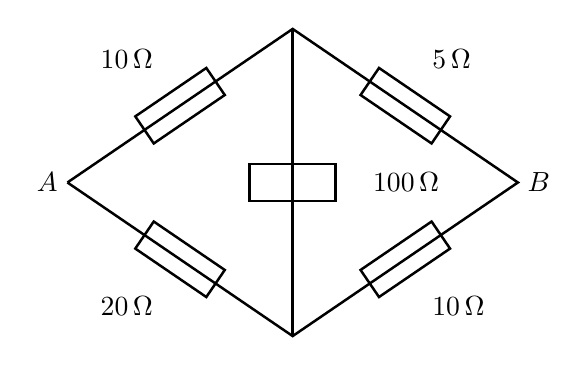
\begin{tikzpicture}[scale=1.3]
  \coordinate (A) at (-2.2,0);
  \coordinate (T) at (0,1.5);
  \coordinate (Bb) at (2.2,0);
  \coordinate (Bo) at (0,-1.5);
  \draw[wire] (A) -- (T) -- (Bb) -- (Bo) -- (A);
  \draw[wire] (T) -- (Bo);
  \node[left] at (A) {$A$};
  \node[right] at (Bb) {$B$};
  % resistor boxes rotated along each edge, centered at midpoint
  \begin{scope}
    \pgfmathsetmacro{\angAT}{atan2(1.5-0,0-(-2.2))}
    \coordinate (mAT) at ($(A)!0.5!(T)$);
    \draw[resistor,rotate around={\angAT:(mAT)}] ($(mAT)+(-0.42,-0.16)$) rectangle ($(mAT)+(0.42,0.16)$);
    \node[above left=1pt] at ($(mAT)+(-0.15,0.25)$) {$10\,\Omega$};
  \end{scope}
  \begin{scope}
    \pgfmathsetmacro{\angTB}{atan2(0-1.5,2.2-0)}
    \coordinate (mTB) at ($(T)!0.5!(Bb)$);
    \draw[resistor,rotate around={\angTB:(mTB)}] ($(mTB)+(-0.42,-0.16)$) rectangle ($(mTB)+(0.42,0.16)$);
    \node[above right=1pt] at ($(mTB)+(0.15,0.25)$) {$5\,\Omega$};
  \end{scope}
  \begin{scope}
    \pgfmathsetmacro{\angABo}{atan2(-1.5-0,0-(-2.2))}
    \coordinate (mABo) at ($(A)!0.5!(Bo)$);
    \draw[resistor,rotate around={\angABo:(mABo)}] ($(mABo)+(-0.42,-0.16)$) rectangle ($(mABo)+(0.42,0.16)$);
    \node[below left=1pt] at ($(mABo)+(-0.15,-0.25)$) {$20\,\Omega$};
  \end{scope}
  \begin{scope}
    \pgfmathsetmacro{\angBoB}{atan2(0-(-1.5),2.2-0)}
    \coordinate (mBoB) at ($(Bo)!0.5!(Bb)$);
    \draw[resistor,rotate around={\angBoB:(mBoB)}] ($(mBoB)+(-0.42,-0.16)$) rectangle ($(mBoB)+(0.42,0.16)$);
    \node[below right=1pt] at ($(mBoB)+(0.15,-0.25)$) {$10\,\Omega$};
  \end{scope}
  % vertical bridge resistor T--Bo
  \resbox{0}{0}{0.42}{}
  \node[right=10pt] at (0.42,0) {$100\,\Omega$};
\end{tikzpicture}
\end{document}
